\label{chap:nram}
In this chapter we will make an overview about the aspects of Neural Random-Access Machines \cite{NRAM:2016} that has as objective the learning of algorithms. The overview starts with a simplified version containing only the registers. It is explained how the pointers manipulation works and later it is explained how the memory-augmented version works.

\section{Registers only model}
The simplified NRAM model can be divided in three main pieces: the controller, which can be a feedforward or a Long-Short Term Memory (LSTM) neural network, the registers and the gates (modules). \newline \newline 
Let $N\ =\ \{0,\ 1,\ 2,\ \dots,\ I - 1\}$ a set of integers, where $I$ is a integer constant. Because the model in \cite{NRAM:2016} should be trained with the gradient descent, the NRAM does not work directly with integers but with probability distributions $p \in \mathbb{R}^{|N|}$, which must satisfy $p_{i} \geq 0$ and $\sum\limits_{i = 0}^{I-1} p_{i} = 1$. Hence, each register or memory cell plays the role of random variable. For instance, let $I = 3$ and $r_1$ a register - the probability distribution contained in $r_1$ associated to the integer 1 is $r_1 = \{0, 1, 0\}$. In this way, the model is fully differentiable.

\subsubsection*{The registers}
The registers is a set of quick access memory cells where each of them contains a vector $p$. The controller does not have a write direct access to the registers, but it can manipulate their values only through the modules.

\subsubsection*{The modules}
In the original paper three types of gates have been introduced: constant, unary and binary. Let $M\ =\ \{m_1, m_2, \dots, m_Q \}$ the set of the modules, then each of them can be represented as a function as follows
\begin{align}
		m_i \in N & \textrm{ (Constant modules)} \\
		m_i: N \rightarrow N & \textrm{ (Unary modules)} \\
		m_i: N \times N \rightarrow N & \textrm{ (Binary modules)}
\end{align}
We use always the same sequence of fourteen modules: Read (described in the Section \ref{sec:nram-memory}), Zero() = 0, One() = 1, Two() = 2, Inc(a) = (a + 1) mod I, Add(a, b) = (a + b) mod I, Sub(a, b) = (a - b) mod I, Dec(a) = (a - 1) mod I, Less-Than(a, b) = [a $\le$ b], Less-Or-Equal-Than(a, b) = [a $\leq$ b], Equal-Than(a, b) = [a = b], Min($a$, $b$) = $\min(a, b)$, Max($a$, $b$) = $\max(a, b)$, Write (described in the Section \ref{sec:nram-memory}). Using always the same sequence is important, because a different permutation of the set M can bring the NRAM to not converge. Furthermore, as for the registers, the gates have to work over probability distributions. Hence, the \textbf{a} and \textbf{b} are vectors which contain probability distributions.

\begin{figure}[t]
	\centering
	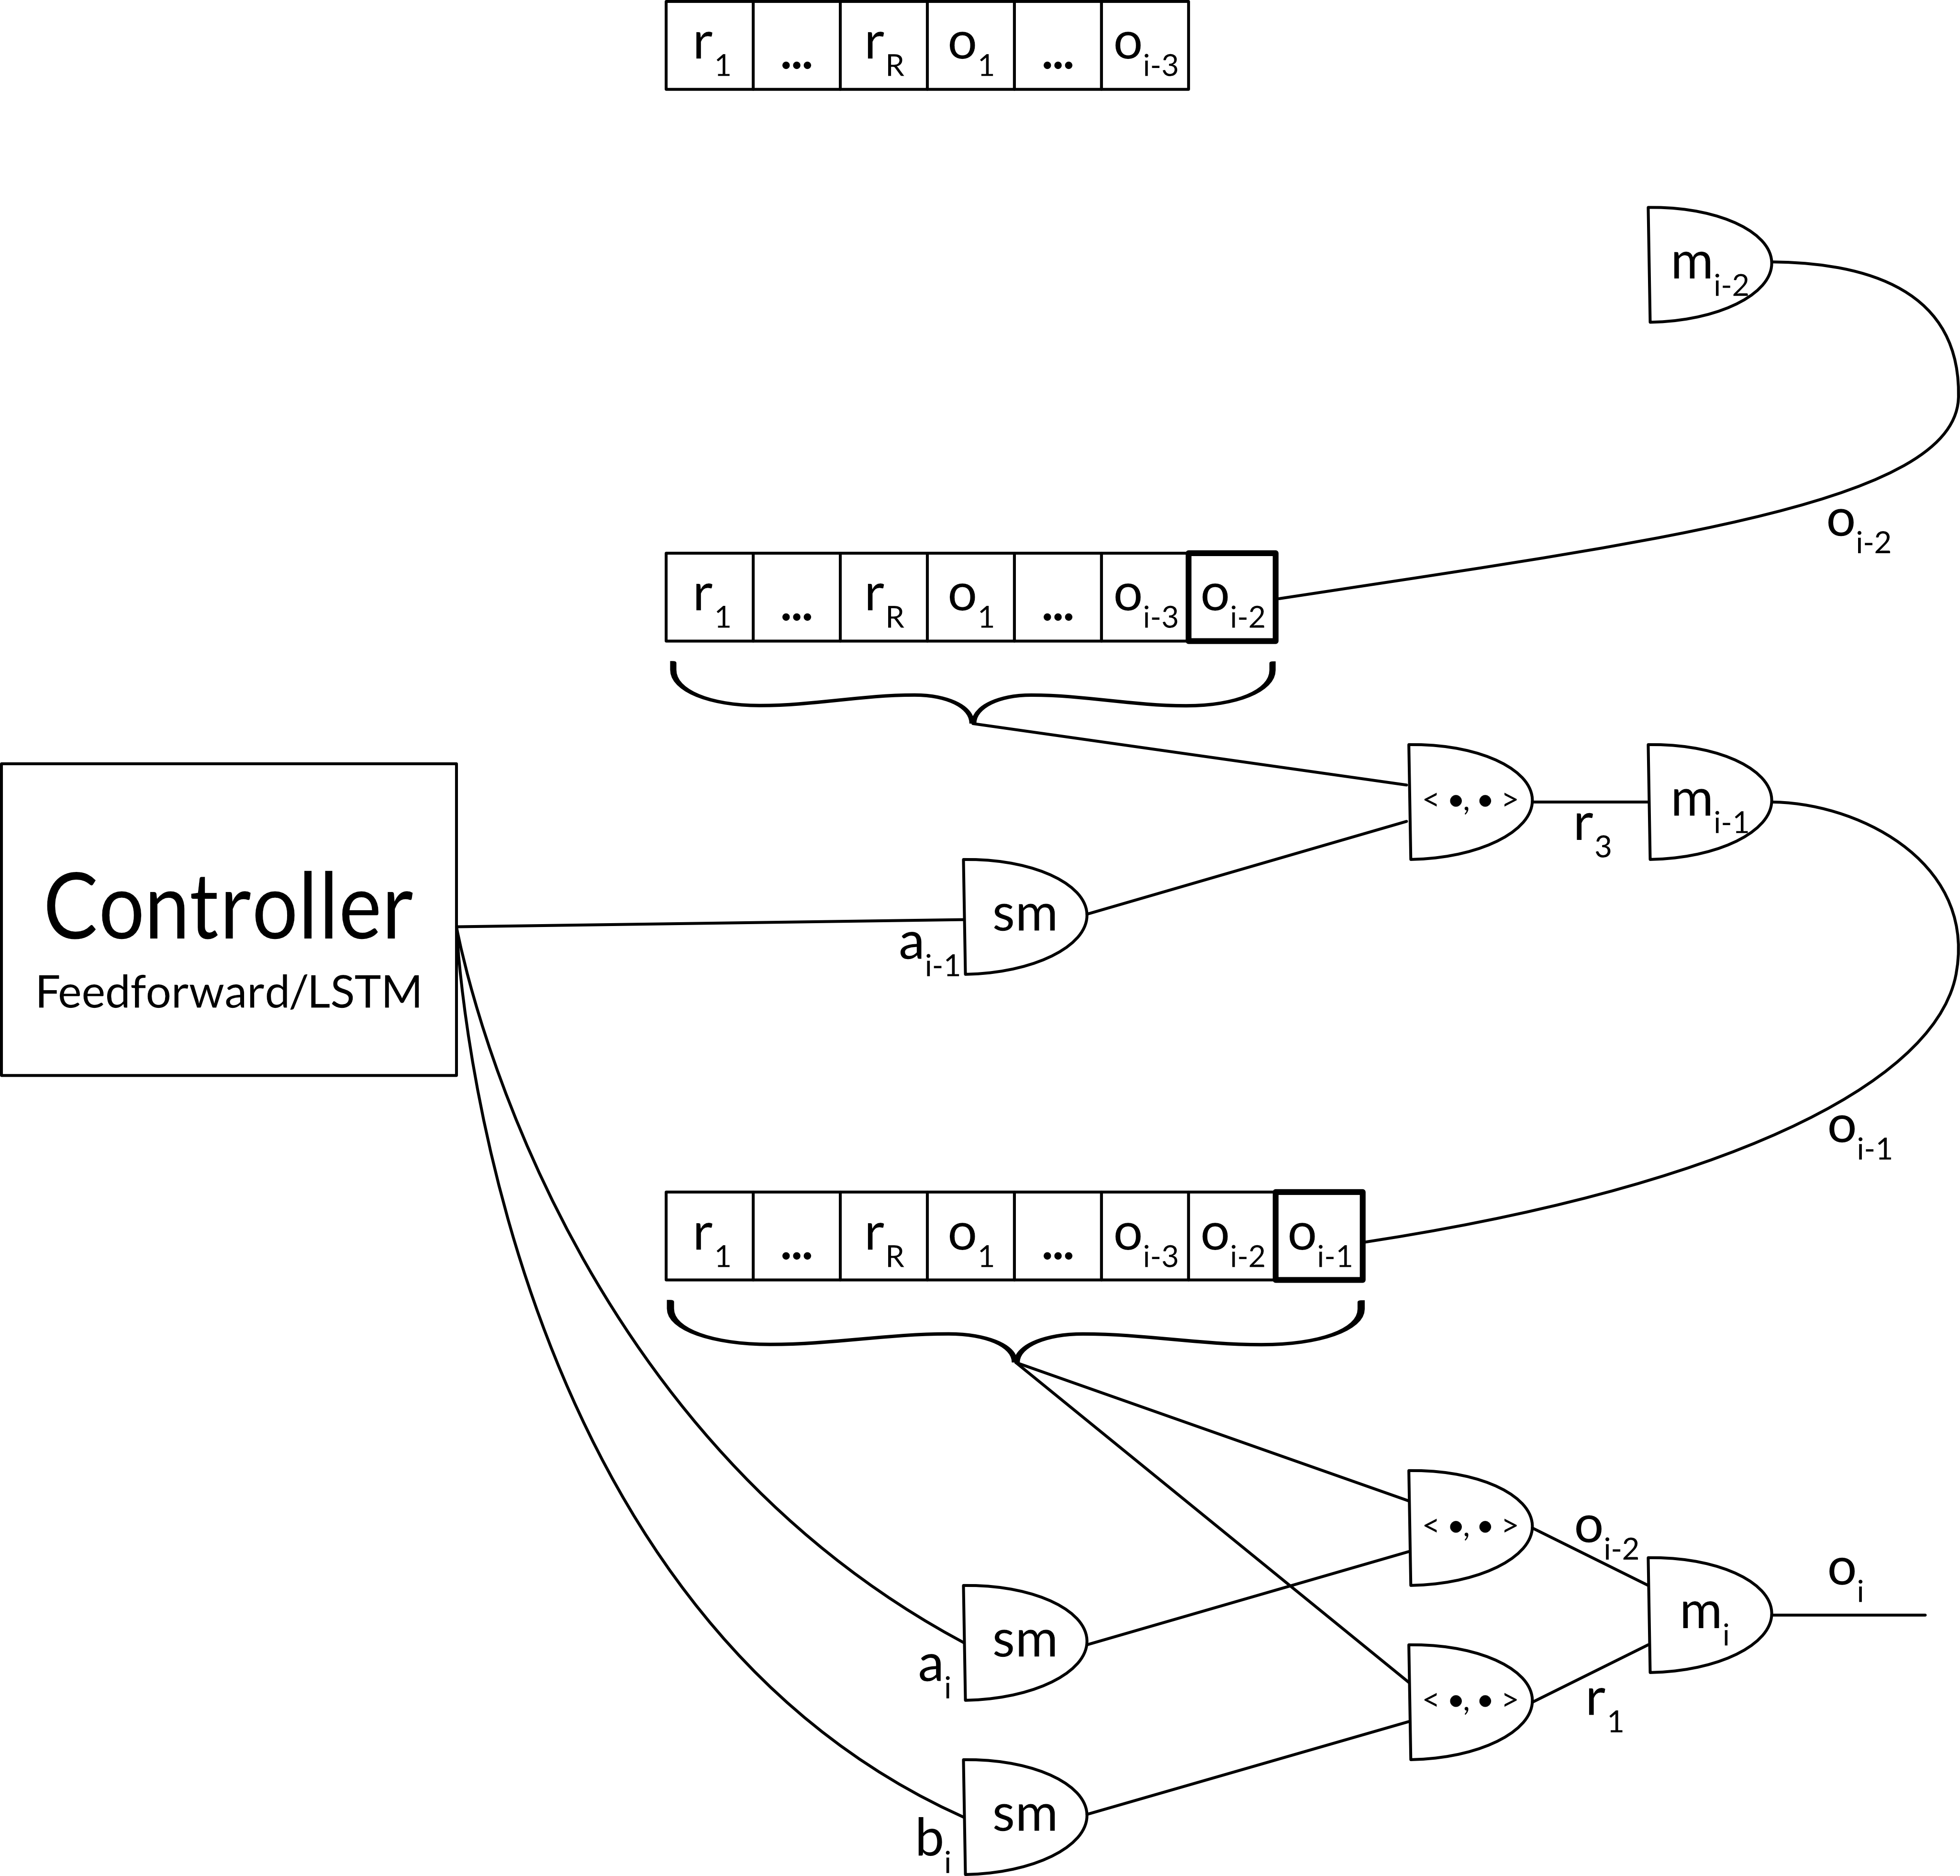
\includegraphics[width=0.6\textwidth]{figures/register-only-model.png}
	\caption{Extract of the execution of the NRAM circuit. The node with \textbf{sm} refers to the softmax activation function, the $<\cdot$, $\cdot>$ to a weighted average between the registers together the output of the previous modules with respect to the \textbf{softmax}($\dots$). With the weighted average the controller selects the data indicated by the coefficient, with which the next module is fed. Here, the gates $m_{i-2},\ m_{i-1},\ m_{i}$ are, respectively, constant, unary and binary.}
	\label{fig:register-only-model}
\end{figure}

\subsection{Execution flow of register-only model}\label{subsec:execution-register-only}
For a better comprehension of the NRAM execution, its pseudocode is visible in the Algorithm \ref{alg:nram}.
\begin{algorithm}
	\begin{algorithmic}[1]
		\State{Let $C$ a controller (MLP or LSTM)}
		\State{Let $R$ the register set}
		\State{Let $M$ a set of modules}
		\State{Let $T$ timesteps}
		\For{each timestep $t \in T$}\label{lst:nram:line-5}
			\State $C$ gets as inputs the $P( x = 0 )$ of the registers\label{lst:nram:line-6}
			\If{$C$ is a LSTM}
				\State $C$ updates its internal state
			\EndIf
			\State $C$ outputs one-shot the configuration of the circuit of the NRAM
			\label{lst:nram:line-8}
			\State The circuit, composed by the set $M$, is executed \label{lst:nram:line-9}
			\State The registers are updated\label{lst:nram:line-10}
		\EndFor
	\end{algorithmic}
	\caption{Execution of the NRAM without the memory}\label{alg:nram}
\end{algorithm}

The execution of the NRAM starts at the Line \ref{lst:nram:line-5} and continue for all the timesteps. At the Line \ref{lst:nram:line-8}, the controller generates a new configuration with the input from the registers, used successively at the Lines \ref{lst:nram:line-9} and \ref{lst:nram:line-10}. The configuration indicates how the circuit is structured, i.e. for each gate indicates the input sources. Hence, in other words, the controller learns how to connect the gates to resolve the problem on which it is trained. In other words, the inputs for the gate $m_i$ are chosen by the controller from the set $\{r_{1}, \dots, r_{R}, o_{1}, \dots, o_{i-1}\}$ where:
\begin{itemize}
	\item $r_j$ is the content of the $j^{th}$ register, $j=1,\dots,R$;
	\item $o_j$ is the output of the $j^{th}$ previous gate with respect to the current $m_i$, $j=1,\dots,|Gates| - 1$.
\end{itemize}
selected through a weighted average with a coefficient as follows
\begin{equation}
	(r_1, r_2, \dots, r_R, o_1, o_2, \dots, o_{i-1})^T\textbf{softmax}(s_i)
\end{equation}
where $\textrm{s}_i \in \mathbb{R}^{R+i-1}$ is a generic vector that indicates the input source for the $i^{th}$ gate. \newline
Hence, let $m_i \in M$ the $i^{th}$ module in $M$, $m_i$ is executed as follows
\begin{itemize}
	\item{Constant gate
		\begin{equation}
			o_i = m_i()
		\end{equation}
	}
	\item{Unary gate
		\begin{equation}
			o_i = m_i((r_1, \dots, r_R, o_1, \dots, o_{i-1})^T\textbf{softmax}(a_i))
		\end{equation}
	}
	\item{Binary gate
		\begin{equation}
			o_i = m_i((r_1, \dots, r_R, o_1, \dots, o_{i-1})^T\textbf{softmax}(a_i), (r_1, \dots, r_R, o_1, \dots, o_{i-1})^T\textbf{softmax}(b_i))
		\end{equation}
	}
\end{itemize}
where, as stated previously, $a_i, b_i \in \mathbb{R}^{R+i-1}$ are produced by the controller and the $o_i$ is the output that is appended to the set $\{r_{1}, \dots, r_{R}, o_{1}, \dots, o_{i-1}\}$ and used later for the subsequent modules.
\begin{figure}[t]
	\centering
	\begin{tikzpicture}[scale=1, node distance = 2.5cm, auto]

		\node [block] (init) {Initialize dataset};
    		\node [block, right of=init, node distance=2.5cm] (emit) {Controller emits the circuit};
    		\node [block, right of=emit, node distance=2.5cm] (circuit) {Circuit is executed};
    		\node [decision, right of=circuit, node distance=3cm] (finish) {t==T or \\ $f_i==1.0$?};
    		\node [round, right of=finish, node distance=3cm] (stop) {Stop};
    		
    		% Void pointer
		\node [coordinate, draw=none, fill=none, below of=finish, node distance=1.5cm] (void_one) {};
		\node [coordinate, draw=none, fill=none, below of=emit, node distance=1.5cm] (void_two) {};    	
    	
    		\draw [->] (init) -- (emit);
    		\draw [->] (emit) -- (circuit);
    		\draw [->] (circuit) -- (finish);
    		\draw [->] (finish) -- node [near start] {yes} (stop);
    		
    		\draw (finish) -- node [near start] {no} (void_one);
    		\draw (void_one) -- node [midway, below] {t = t + 1}  (void_two);
    		
    		\draw [->] (void_two) -- (emit);
    		
	\end{tikzpicture}
	\caption{High level execution of the NRAM without the Curriculum Learning activated. Here, $t$ is a variable which takes into account the current timestep.}
\end{figure}
Since the registers contain probability distributions, the inputs of the modules are also probability distributions because they are weighted averages of probability distributions. Hence, the gates are extended to work over probability distributions and because the inputs are probability distributions also the output is a probability distribution as follows:
\begin{equation}
	P(m_i(A, B) = c) = \sum\limits_{a,b \in N} P(A = a)P(B = b)[m_i(a, b) = c],  for c \in N
\end{equation}
At the same time of the emission of the vectors $a_{i}, b_{i} \in \mathbb{R}^{R+i-1}$, the vectors $c_i \in \mathbb{R}^{R+|M|}$ for $i = 1, 2, \dots, R$  are also emitted, which indicate the sources, that can be the register content at timestep $t-1$ or a module output at the current timestep $t$, from which the new registers content is get. So after the circuit is executed, at the Line \ref{lst:nram:line-10}, the registers content is updated as follows:
\begin{equation}
	r_i^{(t + 1)} = (r_1^{(t)}, \dots, r_R^{(t)}, o_1, \dots, o_{|M|})^T\textbf{softmax}(c_i),\ \ \ i = 1,\dots,R
\end{equation}

As stated previously, at the Line \ref{lst:nram:line-6} the controller gets input from the registers. An easy way would be to give the entire content of the registers, recalling that each of them stores a probability distribution $\mathbb{R}^{I - 1}$. However, in this way the controller cannot generalize to different memory sizes. In fact, as discussed in Section \ref{sec:nram-memory}, the sizes of the memory depends directly on the constant $I$.

\begin{figure}[t!]
	\centering
	
	\begin{tikzpicture}[>=latex',line join=bevel,]
		%%
		\node (R'0) at (389.1bp,84.0bp) [draw,ellipse] {R'0};
  		\node (R'1) at (303.1bp,22.0bp) [draw,ellipse] {R'1};
  		\node (R0) at (20.5bp,78.0bp) [draw,ellipse] {R0};
  		\node (Read) at (105.0bp,78.0bp) [draw,rectangle,ultra thick] {Read};
  		\node (Write) at (212.1bp,22.0bp) [draw,rectangle,ultra thick] {Write};
  		\node (Zero) at (105.0bp,18.0bp) [draw,rectangle,ultra thick] {Zero};
  		\node (Dec) at (303.1bp,84.0bp) [draw,rectangle,ultra thick] {Dec};
  		\node (Inc) at (212.1bp,84.0bp) [draw,rectangle,ultra thick] {Inc};
  		\draw [->] (Dec) ..controls (338.71bp,84.0bp) and (348.04bp,84.0bp)  .. (R'0);
  		\draw [->] (R0) ..controls (49.413bp,78.0bp) and (58.833bp,78.0bp)  .. (Read);
  		\draw [->] (Zero) ..controls (143.07bp,18.275bp) and (155.68bp,18.528bp)  .. (167.1bp,19.0bp) .. controls (169.64bp,19.105bp) and (172.25bp,19.231bp)  .. (Write);
  		\definecolor{strokecol}{rgb}{0.0,0.0,0.0};
  		\pgfsetstrokecolor{strokecol}
  		\draw (158.55bp,26.0bp) node {ptr};
  		\draw [->] (Read) ..controls (144.96bp,80.239bp) and (160.67bp,81.118bp)  .. (Inc);
  		\draw [->] (Write) ..controls (249.28bp,22.0bp) and (260.51bp,22.0bp)  .. (R'1);
  		\draw [->] (Inc) ..controls (247.68bp,84.0bp) and (256.93bp,84.0bp)  .. (Dec);
  		\draw [->] (Read) ..controls (145.35bp,56.905bp) and (161.59bp,48.41bp)  .. (Write);
  		\draw (158.55bp,61.0bp) node {val};
		%
	\end{tikzpicture}
	%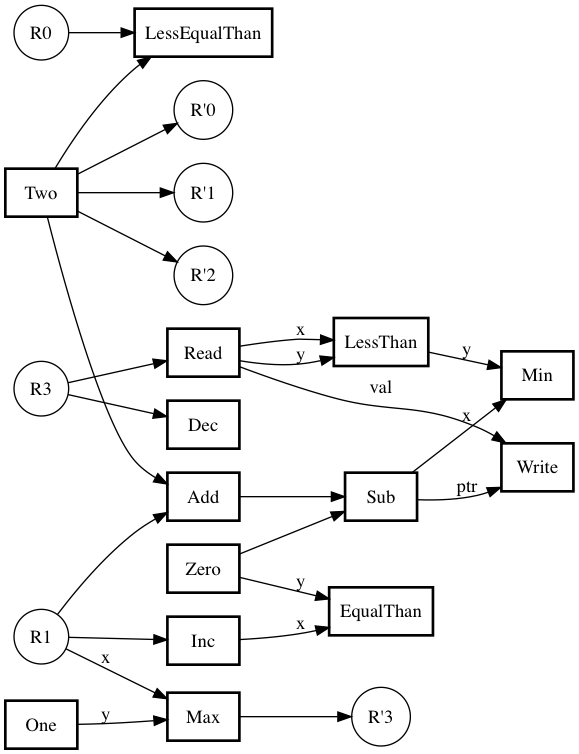
\includegraphics[width=0.5\textwidth]{figures/circuit.png}
	\caption{Example of NRAM circuit. With the circles are represented the registers and with the rectangles are represented the various circuits. The registers with the apex are those that are modified in the timestep. The labels x and y represent the values order for the gates (obviously if it is violated, a gate produces a different result). The modules Read and Write are presented in the next section.}
	\label{fig:example-circuit}
\end{figure}

Hence to resolve this inconvenient, in the original paper the controller receives from all the registers $R$ only $P(r_{i} = 0)$, i.e. the probability that a register content is equal to zero. Another possibility  is to give as input to the controller the discretized registers $r_{i}$ - in other words, what we is done is to discretize the probability distributions, contained in the registers, into integer, using these as input of the controller. Both the solutions limits the information available to the controller, forcing it to solve the problem with the modules instead on its own, and reducing the problem complexity.

%Another possibility that we have experimented is to give as input to the controller the discretized registers $r_{i}$. In other words what we have done is to convert the probability distribution contained in the registers into integer, using these as input of the controller. We have tested and compared this last solution with the original, all the results can be read in the Chapter \ref{experiments}.

\section{Memory augmented model}\label{sec:nram-memory}
The previously described model works only with the registers. Hence, to make that the controller learns an algorithm, the learning process starts initializing the registers with the starting input sequence of the problem. The main disadvantage of this solution is that the model is constrained to the number of the registers, unable to generalize to longer sequence of a problem because, simply, the model cannot process sequences longer than the number of the registers which is constant.\newline\newline
Hence to resolve this problem, the model is augmented with a variable-sized memory tape of $|N|$ memory cells, where each of them stores a distribution over the set $N$. Each distribution both in registers and in memory could be seen as a fuzzy address and so can used by the NRAM as a fuzzy pointer to a memory location. The memory can be formalized as a matrix $\mathcal{M} \in \mathbb{R}_{|N|}^{|N|}$, where a value $\mathcal{M}_{i,j}$ is the probability that the $i^{th}$ memory cell contains the $j^{th}$ integer value.\newline\newline
\begin{figure}[t]
	\centering
	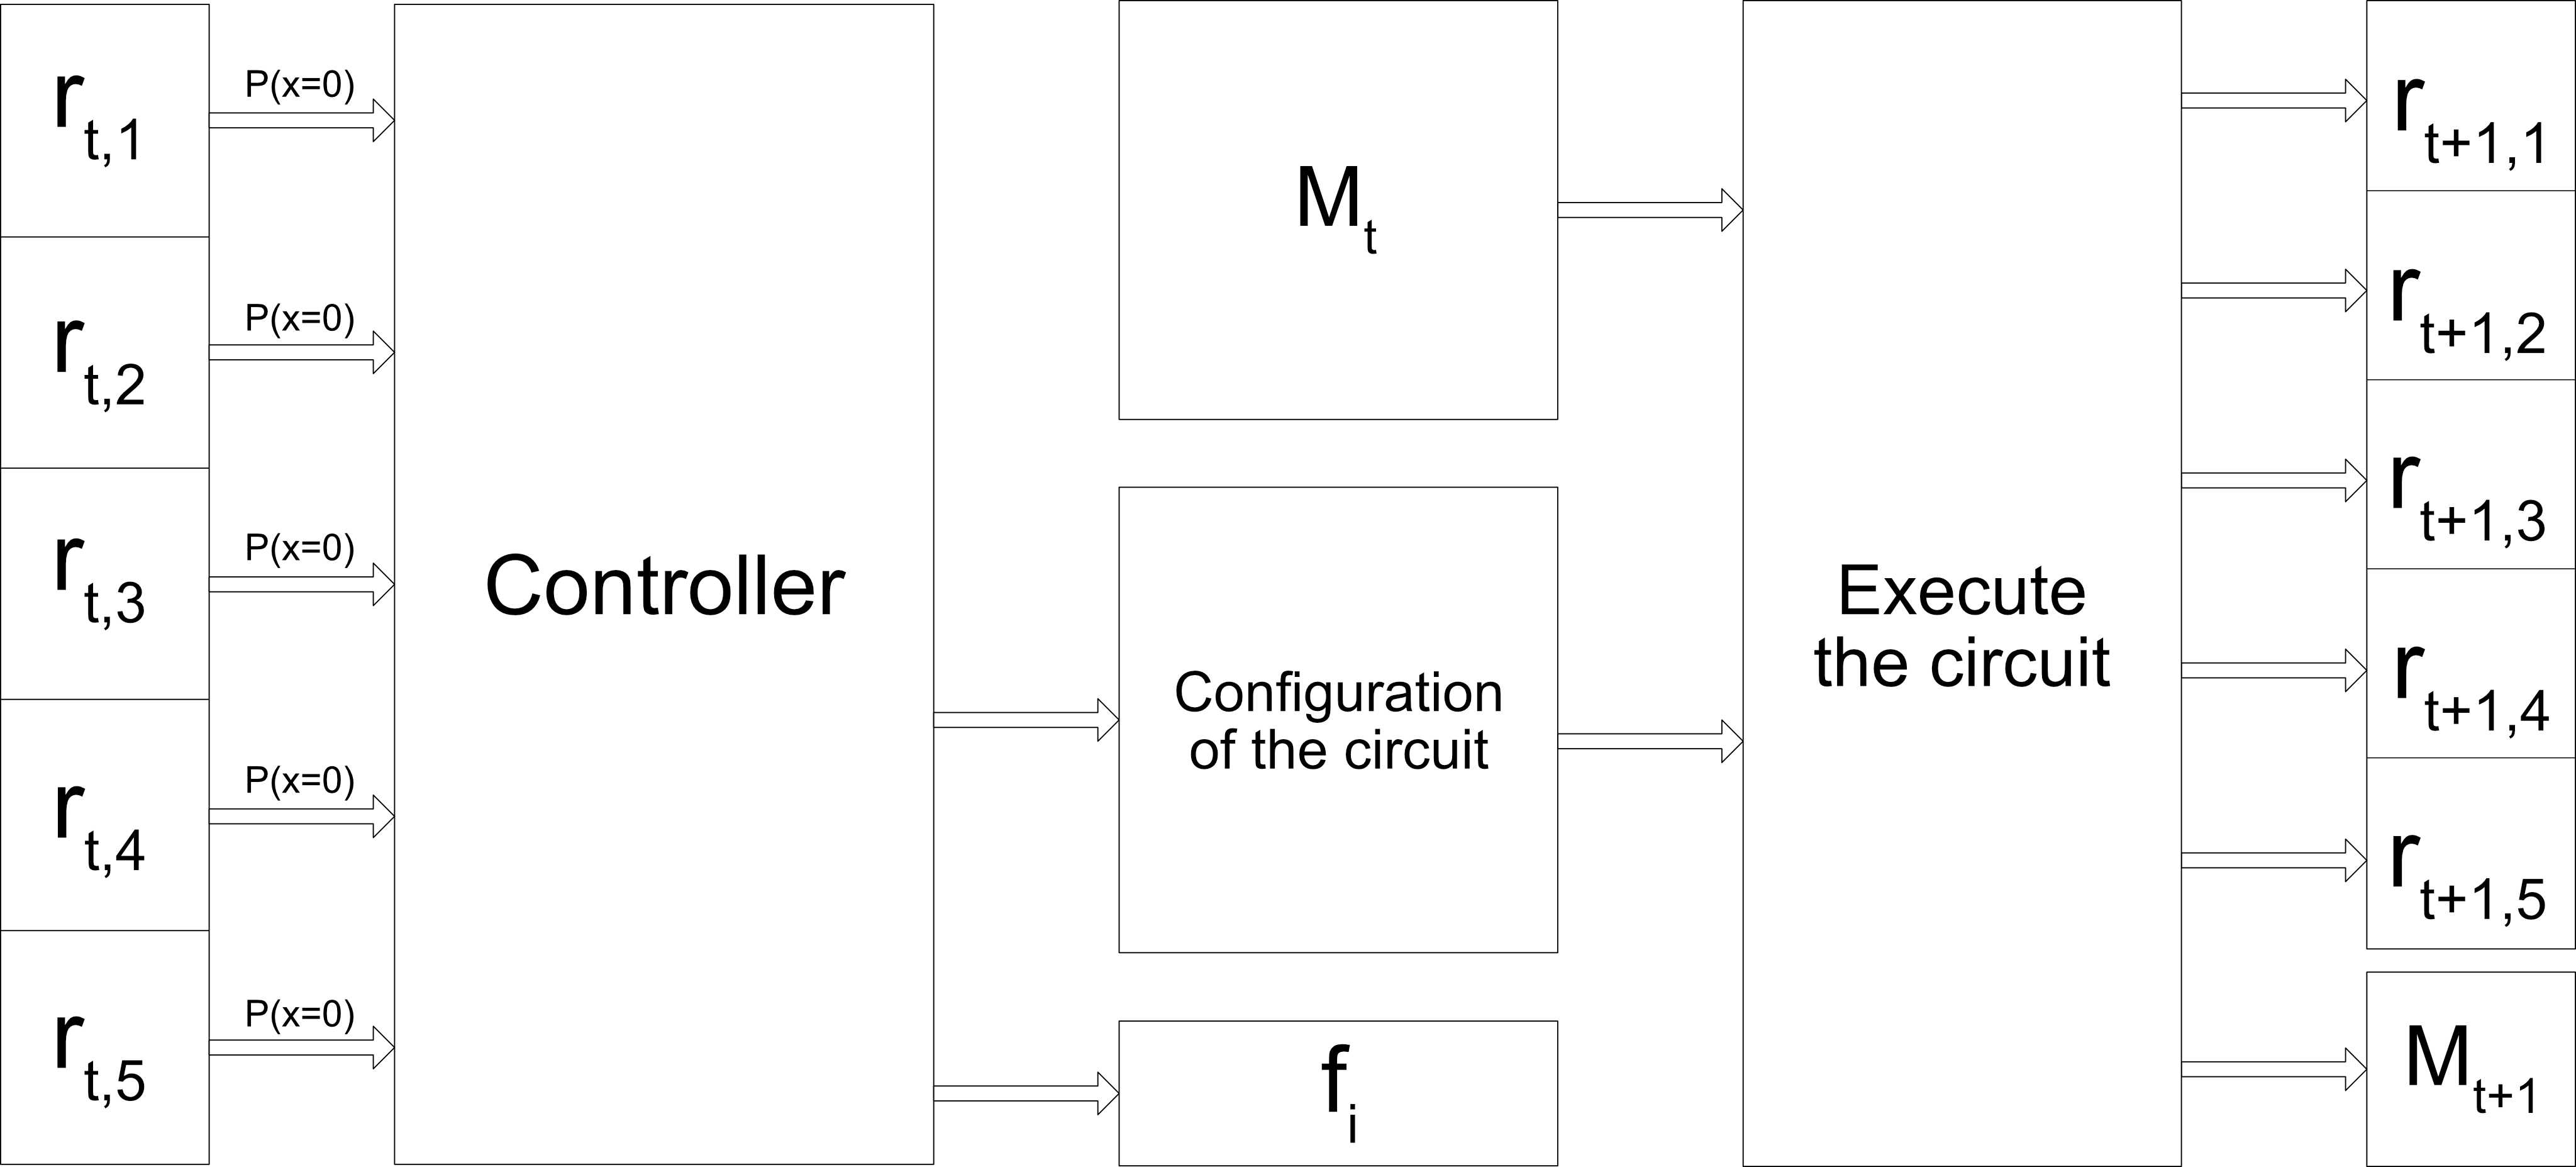
\includegraphics[width=0.8\textwidth]{figures/timestep-nram-execution.png}
	\caption{The execution of the NRAM in a timestep.}
	\label{fig:timestep-nram-execution}
\end{figure}
Hence, to interact with the memory the NRAM contains another two modules:
\begin{itemize}
	\item{\textbf{Read}: this module takes as input a pointer and returns as output the memory content at the location pointed by the pointer. This behaviour is the same when the pointer is an integer or is a probability distribution. More precisely, if the pointer $p\in\mathbb{R}^{|N|}$ is a probability distribution represented as a column vector, then the module returns $\mathcal{M}^{T}p$, while if it is an integer the result is just that cell.}
	\item{\textbf{Write}: this module takes as input a pointer and a value and returns zero. If the inputs are probability distributions the module behave as follows:
\begin{equation}
	\mathcal{M} = (J - p)J^{T} \cdot \mathcal{M} + pa^{T}
\end{equation}
where $J \in \{1\}^{|N|}$ is a column vector and $\cdot$ denotes a coordinate-wise multiplication.}
\end{itemize}
The architecture of the memory augmented NRAM is presented in the Figure \ref{fig:memory-nram}. Recalling the learning process of the registers-only model, in this case the memory is initialized with the problem starting input sequence used as a I/O device. In this way the controller can learn an algorithm operations over a sequence of limited size and later could apply them to a longer sequence.\newline\newline
\begin{figure}[t!]
	\centering
	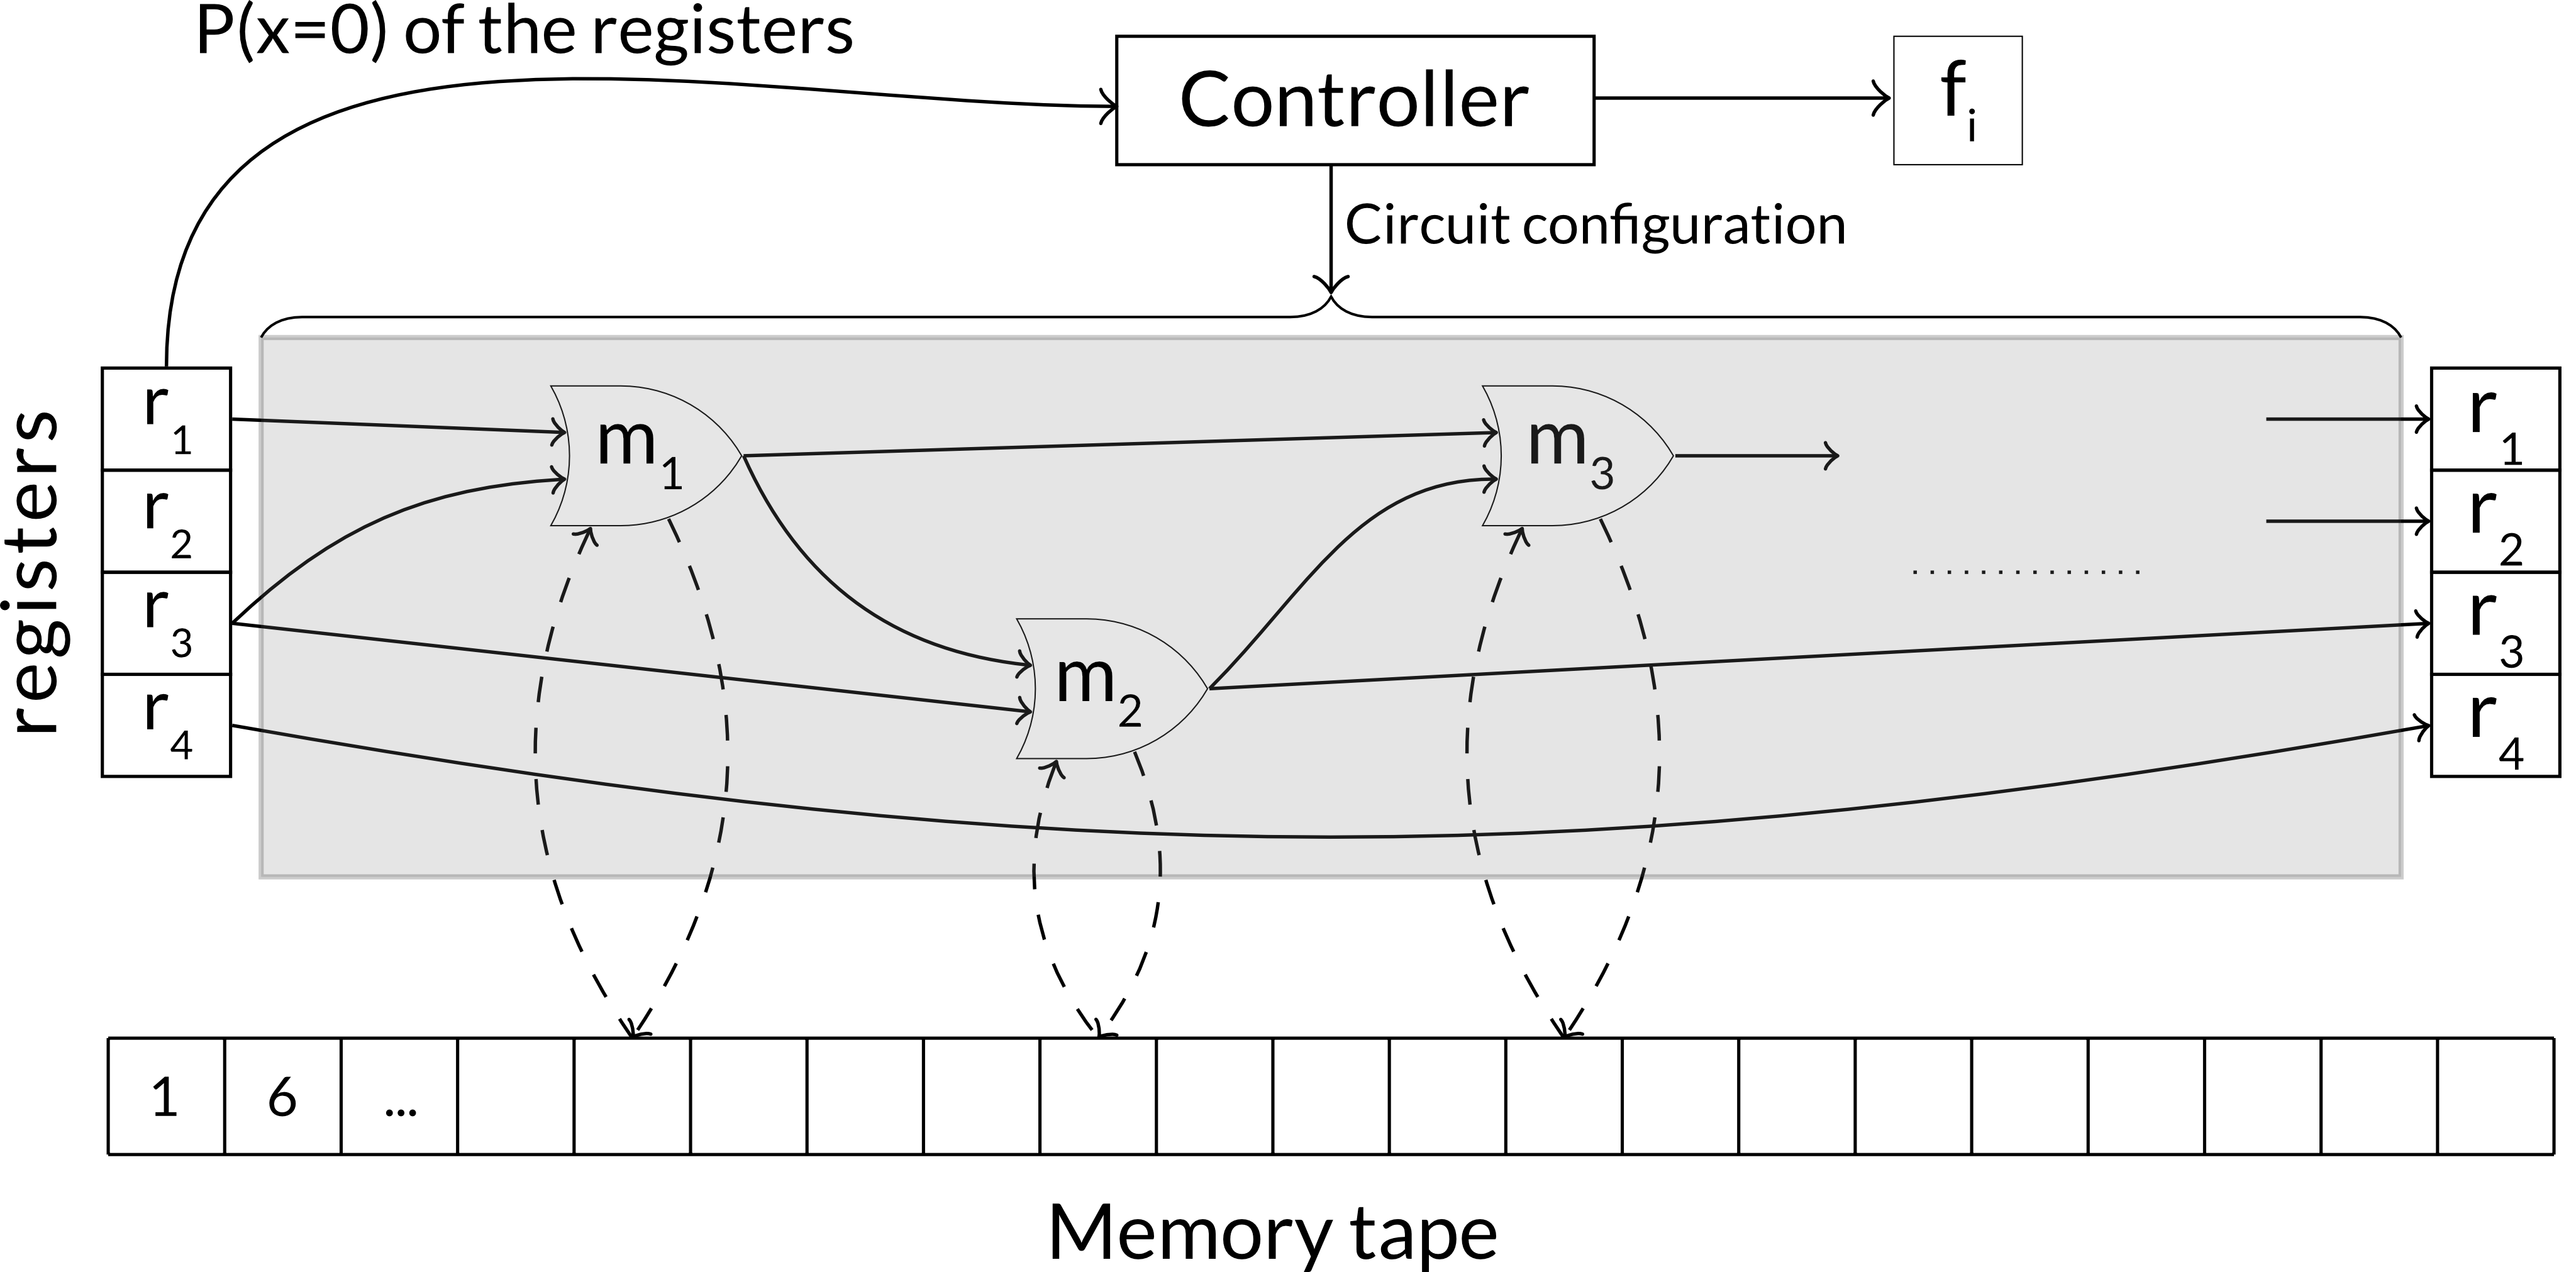
\includegraphics[width=\textwidth]{figures/memory-augmented-model.png}
	\caption{Detailed execution of the NRAM augmented with a memory with $R$ = 4 registers. As can be seen the controller generates the circuit configuration and the $f_i$, starting from the \qq{binarized} version of the registers. Here, that connections are represented with solid lines, except for the interactions with the memory by the \textbf{Read} and \textbf{Write} modules that are represented with dashed lines.}
	\label{fig:memory-nram}
\end{figure}
The NRAM uses a system to decide if the execution can be terminated. Recalling that the execution is divided $T$ timesteps, in each of them the controller emits along the circuit configuration a scalar $f_{t} \in [0, 1]$\footnote{The controller emits a scalar $x_{i}$, with which is produced the $f_i = \textbf{sigmoid}(x_{i})$.}, which represents the willingness of finish the execution in the current timestep $t$. Although in the paper is not explicitly specified, we decided that if $f_{t} = 1.0$ than the execution of NRAM is terminated. Starting from these $f_i$, we have the probability that the execution is not finished in the previous timestep is $\prod\limits_{i=1}^{t-1}(1 - f_{i})$ and the probability that the output is produced in the current timestep is $p_{t} = f_{t} \cdot \prod\limits_{i=1}^{t-1}(1 - f_{i})$. As stated previously, the execution is continued for a maximum of timesteps $T$, except for the previous cases, where the NRAM is forced to emits an output and, due to this, the probability to terminate is $p_{T} = 1 - \sum\limits_{i=1}^{T-1}p_{i}$ regardless of the $f_{T}$ of the last timestep. 

\subsection{Cost function}\label{subsec:cost-function}
Let $\mathcal{M}^{(t)} \in \mathbb{R}^{|N|}_{|N|}$ the memory matrix at the end of the execution of the timestep $t$ and $(x, y) \in N^{|N|}$ a couple which contains the starting input sequence and the expected output sequence, the cost function is defined, only for the memory augmented version, as the expected negative log-likelihood of producing the correct output, i.e.
\begin{equation}
	-\sum\limits_{i=1}^{T}\Bigg(p_{t}\cdot\sum\limits_{i=1}^{|N|}log\Big(\mathcal{M}_{i, y_{i}}^{(t)}\Big)\Bigg)
\end{equation}
where $y_i$ is the expected integer value at the $i^{th}$ memory cell, that here acts also as a pointer. The cost calculation is made only over the part of the memory that contains the output of interest, leaving out the other parts made available as a ``free'' memory which supports the NRAM execution.